\section{Задание}
\[ f(x) = x^2 + 3x + x \ln x \qquad \varepsilon = 10^{-10} \qquad [a, b] = [1, 2] \]

\section{Работа программы}
\begin{figure}[H]
  \centering
  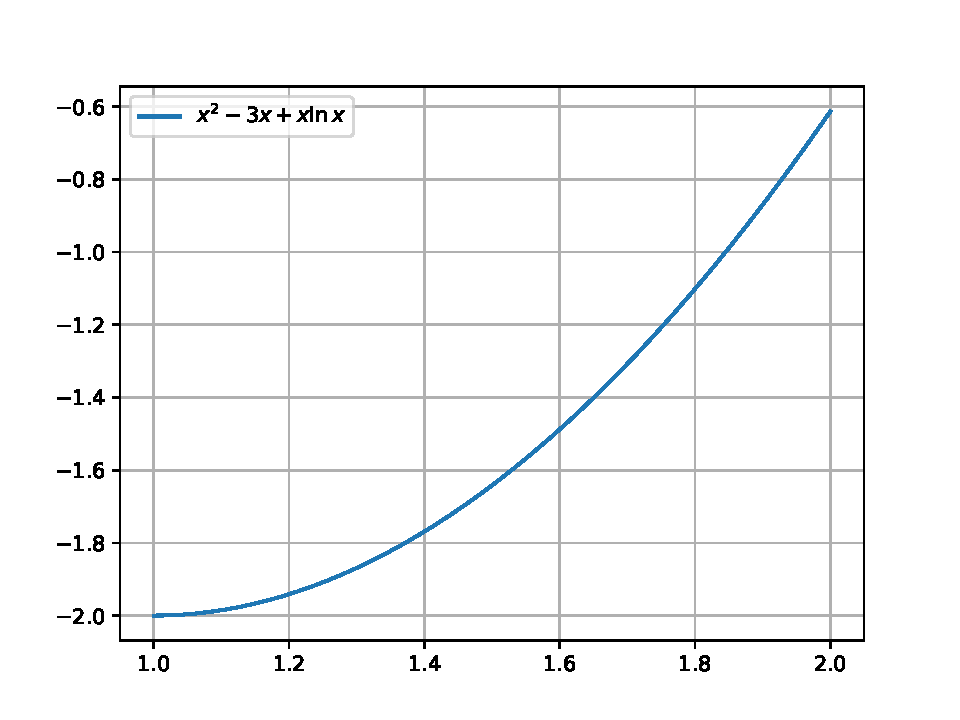
\includegraphics[width=0.8\textwidth]{./img/graph.pdf}
  \caption{График функции}
\end{figure}

\begin{table}[H]
  \centering
  \resizebox{\textwidth}{!}{\begin{tabular}{|l|l|l|l|l|l|l|l|l|}
    \hline
\textnumero & $a$ & $b$ & $x_1$ & $x_2$ & $f(a)$ & $f(b)$ & $f(x_1)$ & $f(x_2)$ \\
    \hline
 1 & 1.00000000000 & 2.00000000000 & 1.49999999995 & 1.50000000005 & -2.00000000000 & -0.61370563888 & -1.64180233791 & -1.64180233777 \\
    \hline
 2 & 1.00000000000 & 1.50000000005 & 1.24999999997 & 1.25000000008 & -2.00000000000 & -1.64180233777 & -1.90857056088 & -1.90857056080 \\
    \hline
 3 & 1.00000000000 & 1.25000000008 & 1.12499999999 & 1.12500000009 & -2.00000000000 & -1.90857056080 & -1.97686908489 & -1.97686908485 \\
    \hline
 4 & 1.00000000000 & 1.12500000009 & 1.06249999999 & 1.06250000009 & -2.00000000000 & -1.97686908485 & -1.99418008932 & -1.99418008930 \\
    \hline
 5 & 1.00000000000 & 1.06250000009 & 1.03125000000 & 1.03125000010 & -2.00000000000 & -1.99418008930 & -1.99854016450 & -1.99854016449 \\
    \hline
 6 & 1.00000000000 & 1.03125000010 & 1.01562500000 & 1.01562500010 & -2.00000000000 & -1.99854016449 & -1.99963441992 & -1.99963441992 \\
    \hline
 7 & 1.00000000000 & 1.01562500010 & 1.00781250000 & 1.00781250010 & -2.00000000000 & -1.99963441992 & -1.99990852643 & -1.99990852643 \\
    \hline
 8 & 1.00000000000 & 1.00781250010 & 1.00390625000 & 1.00390625010 & -2.00000000000 & -1.99990852643 & -1.99997712173 & -1.99997712173 \\
    \hline
 9 & 1.00000000000 & 1.00390625010 & 1.00195312500 & 1.00195312510 & -2.00000000000 & -1.99997712173 & -1.99999427919 & -1.99999427919 \\
    \hline
10 & 1.00000000000 & 1.00195312510 & 1.00097656250 & 1.00097656260 & -2.00000000000 & -1.99999427919 & -1.99999856964 & -1.99999856964 \\
    \hline
11 & 1.00000000000 & 1.00097656260 & 1.00048828125 & 1.00048828135 & -2.00000000000 & -1.99999856964 & -1.99999964239 & -1.99999964239 \\
    \hline
12 & 1.00000000000 & 1.00048828135 & 1.00024414062 & 1.00024414072 & -2.00000000000 & -1.99999964239 & -1.99999991060 & -1.99999991060 \\
    \hline
13 & 1.00000000000 & 1.00024414072 & 1.00012207031 & 1.00012207041 & -2.00000000000 & -1.99999991060 & -1.99999997765 & -1.99999997765 \\
    \hline
14 & 1.00000000000 & 1.00012207041 & 1.00006103516 & 1.00006103526 & -2.00000000000 & -1.99999997765 & -1.99999999441 & -1.99999999441 \\
    \hline
15 & 1.00000000000 & 1.00006103526 & 1.00003051758 & 1.00003051768 & -2.00000000000 & -1.99999999441 & -1.99999999860 & -1.99999999860 \\
    \hline
16 & 1.00000000000 & 1.00003051768 & 1.00001525879 & 1.00001525889 & -2.00000000000 & -1.99999999860 & -1.99999999965 & -1.99999999965 \\
    \hline
17 & 1.00000000000 & 1.00001525889 & 1.00000762939 & 1.00000762949 & -2.00000000000 & -1.99999999965 & -1.99999999991 & -1.99999999991 \\
    \hline
18 & 1.00000000000 & 1.00000762949 & 1.00000381470 & 1.00000381480 & -2.00000000000 & -1.99999999991 & -1.99999999998 & -1.99999999998 \\
    \hline
19 & 1.00000000000 & 1.00000381480 & 1.00000190735 & 1.00000190745 & -2.00000000000 & -1.99999999998 & -1.99999999999 & -1.99999999999 \\
    \hline
20 & 1.00000000000 & 1.00000190745 & 1.00000095367 & 1.00000095377 & -2.00000000000 & -1.99999999999 & -2.00000000000 & -2.00000000000 \\
    \hline
21 & 1.00000095367 & 1.00000190745 & 1.00000143051 & 1.00000143061 & -2.00000000000 & -1.99999999999 & -2.00000000000 & -2.00000000000 \\
    \hline
22 & 1.00000095367 & 1.00000143061 & 1.00000119209 & 1.00000119219 & -2.00000000000 & -2.00000000000 & -2.00000000000 & -2.00000000000 \\
    \hline
23 & 1.00000095367 & 1.00000119219 & 1.00000107288 & 1.00000107298 & -2.00000000000 & -2.00000000000 & -2.00000000000 & -2.00000000000 \\
    \hline
24 & 1.00000107288 & 1.00000119219 & 1.00000113249 & 1.00000113259 & -2.00000000000 & -2.00000000000 & -2.00000000000 & -2.00000000000 \\
    \hline
25 & 1.00000107288 & 1.00000113259 & 1.00000110269 & 1.00000110279 & -2.00000000000 & -2.00000000000 & -2.00000000000 & -2.00000000000 \\
    \hline
  \end{tabular}}
  \caption{Результат работы метода половинного деления}
\end{table}

Ответ, полученный с помощью метода половинного деления:
\[
  x_\min = 1.00000110274
  \qquad
  f(x_{\min}) = -2.00000000000
\]

\begin{table}[H]
  \resizebox{\textwidth}{!}{\begin{tabular}{|l|l|l|l|l|l|l|l|l|}
    \hline
\textnumero & $a$ & $b$ & $x_1$ & $x_2$ & $f(a)$ & $f(b)$ & $f(x_1)$ & $f(x_2)$ \\
    \hline
 1 & 1.00000000000 & 2.00000000000 & 1.38196601125 & 1.61803398875 & -2.00000000000 & -0.61370563888 & -1.78899211784 & -1.45745088876 \\
    \hline
 2 & 1.00000000000 & 1.61803398875 & 1.23606797750 & 1.38196601125 & -2.00000000000 & -1.45745088876 & -1.91837338126 & -1.78899211784 \\
    \hline
 3 & 1.00000000000 & 1.38196601125 & 1.14589803375 & 1.23606797750 & -2.00000000000 & -1.78899211784 & -1.96855350437 & -1.91837338126 \\
    \hline
 4 & 1.00000000000 & 1.23606797750 & 1.09016994375 & 1.14589803375 & -2.00000000000 & -1.91837338126 & -1.98792103373 & -1.96855350437 \\
    \hline
 5 & 1.00000000000 & 1.14589803375 & 1.05572809000 & 1.09016994375 & -2.00000000000 & -1.96855350437 & -1.99536963720 & -1.98792103373 \\
    \hline
 6 & 1.00000000000 & 1.09016994375 & 1.03444185375 & 1.05572809000 & -2.00000000000 & -1.98792103373 & -1.99822733256 & -1.99536963720 \\
    \hline
 7 & 1.00000000000 & 1.05572809000 & 1.02128623625 & 1.03444185375 & -2.00000000000 & -1.99536963720 & -1.99932193481 & -1.99822733256 \\
    \hline
 8 & 1.00000000000 & 1.03444185375 & 1.01315561750 & 1.02128623625 & -2.00000000000 & -1.99822733256 & -1.99974077159 & -1.99932193481 \\
    \hline
 9 & 1.00000000000 & 1.02128623625 & 1.00813061876 & 1.01315561750 & -2.00000000000 & -1.99932193481 & -1.99990092878 & -1.99974077159 \\
    \hline
10 & 1.00000000000 & 1.01315561750 & 1.00502499874 & 1.00813061876 & -2.00000000000 & -1.99974077159 & -1.99996214518 & -1.99990092878 \\
    \hline
11 & 1.00000000000 & 1.00813061876 & 1.00310562002 & 1.00502499874 & -2.00000000000 & -1.99990092878 & -1.99998553767 & -1.99996214518 \\
    \hline
12 & 1.00000000000 & 1.00502499874 & 1.00191937873 & 1.00310562002 & -2.00000000000 & -1.99996214518 & -1.99999447516 & -1.99998553767 \\
    \hline
13 & 1.00000000000 & 1.00310562002 & 1.00118624129 & 1.00191937873 & -2.00000000000 & -1.99998553767 & -1.99999788953 & -1.99999447516 \\
    \hline
14 & 1.00000000000 & 1.00191937873 & 1.00073313744 & 1.00118624129 & -2.00000000000 & -1.99999447516 & -1.99999919383 & -1.99999788953 \\
    \hline
15 & 1.00000000000 & 1.00118624129 & 1.00045310385 & 1.00073313744 & -2.00000000000 & -1.99999788953 & -1.99999969206 & -1.99999919383 \\
    \hline
16 & 1.00000000000 & 1.00073313744 & 1.00028003358 & 1.00045310385 & -2.00000000000 & -1.99999919383 & -1.99999988238 & -1.99999969206 \\
    \hline
17 & 1.00000000000 & 1.00045310385 & 1.00017307027 & 1.00028003358 & -2.00000000000 & -1.99999969206 & -1.99999995507 & -1.99999988238 \\
    \hline
18 & 1.00000000000 & 1.00028003358 & 1.00010696331 & 1.00017307027 & -2.00000000000 & -1.99999988238 & -1.99999998284 & -1.99999995507 \\
    \hline
19 & 1.00000000000 & 1.00017307027 & 1.00006610696 & 1.00010696331 & -2.00000000000 & -1.99999995507 & -1.99999999344 & -1.99999998284 \\
    \hline
20 & 1.00000000000 & 1.00010696331 & 1.00004085635 & 1.00006610696 & -2.00000000000 & -1.99999998284 & -1.99999999750 & -1.99999999344 \\
    \hline
21 & 1.00000000000 & 1.00006610696 & 1.00002525061 & 1.00004085635 & -2.00000000000 & -1.99999999344 & -1.99999999904 & -1.99999999750 \\
    \hline
22 & 1.00000000000 & 1.00004085635 & 1.00001560574 & 1.00002525061 & -2.00000000000 & -1.99999999750 & -1.99999999963 & -1.99999999904 \\
    \hline
23 & 1.00000000000 & 1.00002525061 & 1.00000964488 & 1.00001560574 & -2.00000000000 & -1.99999999904 & -1.99999999986 & -1.99999999963 \\
    \hline
24 & 1.00000000000 & 1.00001560574 & 1.00000596086 & 1.00000964488 & -2.00000000000 & -1.99999999963 & -1.99999999995 & -1.99999999986 \\
    \hline
25 & 1.00000000000 & 1.00000964488 & 1.00000368401 & 1.00000596086 & -2.00000000000 & -1.99999999986 & -1.99999999998 & -1.99999999995 \\
    \hline
  \end{tabular}}
  \caption{Результат работы метода золотого сечения}
\end{table}
\[
  x_\min = 1.00000482244
  \qquad
  f(x_{\min}) = -1.99999999997
\]

\begin{table}[H]
  \centering
  \begin{tabular}{|l|l|l|l|l|}
\hline
    \textnumero & $x$ & $f(x)$ & $f'(x)$ & $f''(x)$ \\
\hline
 1 & 1.5000E+00 & -1.6418E+00 & 1.4055E+00 & 2.6667E+00 \\
\hline
 2 & 9.7295E-01 & -1.9989E+00 & -8.1521E-02 & 3.0278E+00 \\
\hline
 3 & 9.9987E-01 & -2.0000E+00 & -3.7597E-04 & 3.0001E+00 \\
\hline
 4 & 1.0000E+00 & -2.0000E+00 & -7.8535E-09 & 3.0000E+00 \\
\hline
 5 & 1.0000E+00 & -2.0000E+00 & 0.0000E+00 & 3.0000E+00 \\
\hline
  \end{tabular}
\end{table}
\[
  x_\min = 1.00000000000
  \qquad
  f(x_{\min}) = -2.00000000000
\]

\clearpage
\section{Исходный код}
\inputminted[breaklines]{Python}{../solution.py}
